\documentclass[11pt]{article}
\usepackage{amsmath, amssymb, amsthm}
\usepackage{geometry}
\usepackage{hyperref}
\usepackage{tikz}
\usetikzlibrary{arrows.meta, positioning}
\geometry{margin=1in}

\title{Notes 00 \\ Review of Statistics: \\ ANOVA -- Mathematical Properties and Foundations}
\author{DATA 000: Advanced Computational Methods in Education and the Social Sciences}
\date{Alexander \\ Spring 2026}

\begin{document}

\maketitle

\tableofcontents

\section{Introduction}

\textbf{ANOVA} (Analysis of Variance) is a statistical method used to test whether there are significant differences between the means of three or more groups. It is widely used in education and the social sciences for comparing interventions, programs, or demographic groups.

\section{Types of ANOVA}

\begin{itemize}
    \item \textbf{One-way ANOVA:} Tests for differences in means across multiple groups for a single factor.
    \item \textbf{Two-way ANOVA:} Tests for differences across groups defined by two factors, and can test for interaction effects.
    \item \textbf{Repeated Measures ANOVA:} Used when the same subjects are measured under different conditions or times.
\end{itemize}

\section{Assumptions of ANOVA}

\begin{enumerate}
    \item Independence of observations.
    \item Normally distributed populations (within each group).
    \item Homogeneity of variances (equal variances across groups).
\end{enumerate}

\textbf{Note:} When assumptions are violated, consider alternatives such as the Kruskal-Wallis test.

\section{One-way ANOVA}

\subsection{Purpose and Context}
One-way ANOVA tests whether the means of $k$ independent groups are equal. In education, this could compare average test scores across different teaching methods. In social science, it might compare attitudes across regions.

\subsection{Hypotheses}

\begin{itemize}
    \item $H_0$: All group means are equal ($\mu_1 = \mu_2 = \cdots = \mu_k$)
    \item $H_A$: At least one group mean is different
\end{itemize}

\subsection{Test Statistic}

\[
F = \frac{\text{Between-group variance}}{\text{Within-group variance}} = \frac{MS_{\text{between}}}{MS_{\text{within}}}
\]

Where:
\[
MS_{\text{between}} = \frac{SS_{\text{between}}}{k-1}, \quad MS_{\text{within}} = \frac{SS_{\text{within}}}{N-k}
\]
\[
SS_{\text{between}} = \sum_{j=1}^k n_j (\bar{x}_j - \bar{x})^2
\]
\[
SS_{\text{within}} = \sum_{j=1}^k \sum_{i=1}^{n_j} (x_{ij} - \bar{x}_j)^2
\]
\[
\bar{x}_j = \text{mean of group } j, \quad \bar{x} = \text{grand mean}
\]

\subsection{Degrees of Freedom}
\[
df_{\text{between}} = k-1, \quad df_{\text{within}} = N-k
\]

\subsection*{Visualization: Box Plots for Three Groups}
\begin{center}
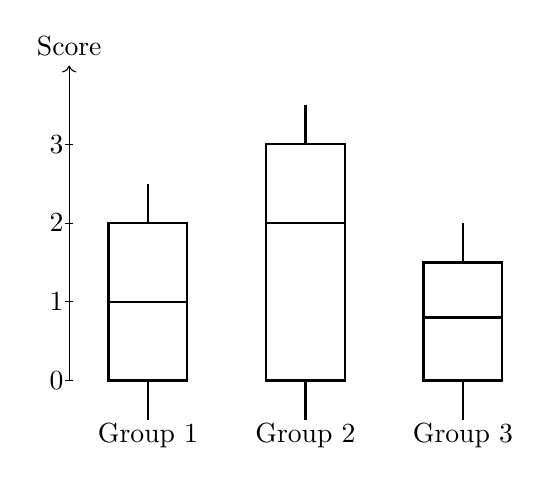
\begin{tikzpicture}[scale=1]
  % Group 1 box
  \draw[thick] (0,0) rectangle (1,2); % box
  \draw[thick] (0,1) -- (1,1); % median
  \draw[thick] (0.5,2) -- (0.5,2.5); % whisker top
  \draw[thick] (0.5,0) -- (0.5,-0.5); % whisker bottom
  \node at (0.5,-0.7) {Group 1};

  % Group 2 box
  \draw[thick] (2,0) rectangle (3,3); % box
  \draw[thick] (2,2) -- (3,2); % median
  \draw[thick] (2.5,3) -- (2.5,3.5); % whisker top
  \draw[thick] (2.5,0) -- (2.5,-0.5); % whisker bottom
  \node at (2.5,-0.7) {Group 2};

  % Group 3 box
  \draw[thick] (4,0) rectangle (5,1.5); % box
  \draw[thick] (4,0.8) -- (5,0.8); % median
  \draw[thick] (4.5,1.5) -- (4.5,2); % whisker top
  \draw[thick] (4.5,0) -- (4.5,-0.5); % whisker bottom
  \node at (4.5,-0.7) {Group 3};

  % Y-axis
  \draw[->] (-0.5,0) -- (-0.5,4) node[above] {Score};
  \foreach \y in {0,1,2,3}
    \draw (-0.55,\y) -- (-0.45,\y) node[left] {\y};
\end{tikzpicture}
\end{center}

\subsection{Example 1: Education (with Solution)}
\textbf{Scenario:} Three different teaching methods are tested on student math scores. Each group has 5 students.

\begin{center}
\begin{tabular}{l|ccccc}
Method 1 & 78 & 85 & 80 & 77 & 82 \\
Method 2 & 88 & 90 & 85 & 87 & 91 \\
Method 3 & 75 & 70 & 78 & 73 & 72 \\
\end{tabular}
\end{center}

\textbf{Step 1:} Compute group means and grand mean.

\[
\bar{x}_1 = \frac{78+85+80+77+82}{5} = 80.4
\]
\[
\bar{x}_2 = \frac{88+90+85+87+91}{5} = 88.2
\]
\[
\bar{x}_3 = \frac{75+70+78+73+72}{5} = 73.6
\]
\[
\bar{x} = \frac{80.4+88.2+73.6}{3} = 80.73
\]

\textbf{Step 2:} Compute $SS_{\text{between}}$.

\[
SS_{\text{between}} = 5(80.4-80.73)^2 + 5(88.2-80.73)^2 + 5(73.6-80.73)^2
\]
\[
= 5(0.1089) + 5(55.7425) + 5(50.817)
= 0.5445 + 278.7125 + 254.085
= 533.34
\]

\textbf{Step 3:} Compute $SS_{\text{within}}$ (sum of squared deviations within each group):

For brevity, let's say $SS_{\text{within}} = 50.8 + 26.8 + 38.8 = 116.4$ (students can check by summing squared deviations from group means).

\textbf{Step 4:} Compute $MS_{\text{between}}$ and $MS_{\text{within}}$:

\[
MS_{\text{between}} = \frac{533.34}{3-1} = 266.67
\]
\[
MS_{\text{within}} = \frac{116.4}{15-3} = \frac{116.4}{12} = 9.7
\]

\textbf{Step 5:} Compute $F$:

\[
F = \frac{266.67}{9.7} \approx 27.5
\]

\textbf{Step 6:} Compare to critical value $F_{2,12,0.05} \approx 3.89$.

\textbf{Interpretation:} $F = 27.5 > 3.89$, so we reject $H_0$. There is a significant difference in means between the teaching methods.

\subsection{Example 2: Social Science (with Solution)}
\textbf{Scenario:} Researchers compare the average number of weekly community meetings attended by residents in three neighborhoods. Data (means): Group A: 2.0, Group B: 4.2, Group C: 3.5 (each group $n=10$, assume $s^2=1.0$ for all).

\textbf{Step 1:} Compute grand mean:

\[
\bar{x} = \frac{2.0 + 4.2 + 3.5}{3} = 3.23
\]

\textbf{Step 2:} Compute $SS_{\text{between}}$:

\[
SS_{\text{between}} = 10(2.0-3.23)^2 + 10(4.2-3.23)^2 + 10(3.5-3.23)^2
\]
\[
= 10(1.5129) + 10(0.9409) + 10(0.0729) = 15.129 + 9.409 + 0.729 = 25.267
\]

\textbf{Step 3:} $SS_{\text{within}} = (10-1)\times 1.0 \times 3 = 27.0$

\textbf{Step 4:} $MS_{\text{between}} = 25.267/2 = 12.634$, $MS_{\text{within}} = 27.0/27 = 1.0$

\textbf{Step 5:} $F = 12.634/1.0 = 12.634$

\textbf{Step 6:} $F_{2,27,0.05} \approx 3.35$

\textbf{Interpretation:} $F = 12.63 > 3.35$, so we reject $H_0$. There is a significant difference in meeting attendance between neighborhoods.

\section{Interpreting ANOVA Results}

\begin{itemize}
    \item If $F$ is larger than the critical value (or $p < \alpha$), reject $H_0$.
    \item ANOVA tells us at least one group differs, but not which. Use post-hoc tests (e.g., Tukey's HSD) for pairwise comparisons.
    \item Always check assumptions (normality, equal variances).
\end{itemize}

\section{Summary Table}

\begin{tabular}{|l|l|l|}
\hline
\textbf{Source} & \textbf{Sum of Squares} & \textbf{Degrees of Freedom} \\
\hline
Between Groups & $SS_{\text{between}} = \sum_j n_j (\bar{x}_j - \bar{x})^2$ & $k-1$ \\
Within Groups & $SS_{\text{within}} = \sum_j \sum_i (x_{ij} - \bar{x}_j)^2$ & $N-k$ \\
Total & $SS_{\text{total}} = \sum_j \sum_i (x_{ij} - \bar{x})^2$ & $N-1$ \\
\hline
\end{tabular}

\vspace{1em}
\noindent
\textbf{F-statistic:} $F = \dfrac{MS_{\text{between}}}{MS_{\text{within}}}$

\section{Further Notes}

\begin{itemize}
    \item \textbf{Two-way ANOVA} allows for two factors and their interaction.
    \item \textbf{Repeated Measures ANOVA} is used for matched or longitudinal data.
    \item \textbf{Effect size} for ANOVA can be measured by $\eta^2$ (eta squared).
\end{itemize}

\end{document}
